\subsection{Errors}
\label{sec:errors}
The collected charge is calculated using \ref{eq:capacitance}, hence
\begin{equation}
  \label{eq:uncertainties}
  \delta Q = \sqrt{(\delta C)^2 + (\delta V)^2}.
\end{equation}
The capacitance of the pre-amplifier was given in \autocite{LabInstruction}
without uncertainty so, to be conservative, we will assume $\delta C =
0.5$~pF. The high voltage power supply (HVPS) was used to adjust and read the
input, the sensitivity of the instrument is $\pm$ 1~V, thus $\delta V = 1$~V.

The relationship between the HV:
\begin{equation}
  U_{HV(U_{ref})} = \alpha U_{ref} + \beta
\end{equation}
from where we can get the error as:
\begin{equation}
  \delta U_{HV(U_{ref})} = \sqrt{ (\delta \alpha  U_{ref})^2 + (\delta \beta)^2 + (\alpha \delta U_{ref})^2 }
\end{equation}
The charge collected in the anode was obtained feeding the input of the
preamplifier with a square pulse and measuring the MCA response.
\begin{equation}
  Q = C U_{pulse (N)}
\end{equation}
Where Q is the charge collected, the C capacitance and N is the multichannel
analyzer response that depends lineary on the gain chosen.
\begin{equation}
  U_{pulse (N)}= C\alpha_G N_G + \beta_G
\end{equation}
Hence the error for Q would be:
\begin{equation}
  \delta Q = \sqrt{(\delta CU_p )^2 + (C \sqrt{(N\delta \alpha)^2+(\delta \beta)^2} )^2 + (C\alpha \delta N)^2}
\end{equation}
On the resolution side most errors treated and obtained from the Gaussian
distribution
\begin{equation}
  \delta R = \sqrt{(\frac{\delta \sigma,}{\sigma})^2 + (\frac{\delta \mu}{\mu})^2}
\end{equation}
\begin{figure}[!h]
  \centering
  \begin{subfigure}[t]{.48\linewidth}
    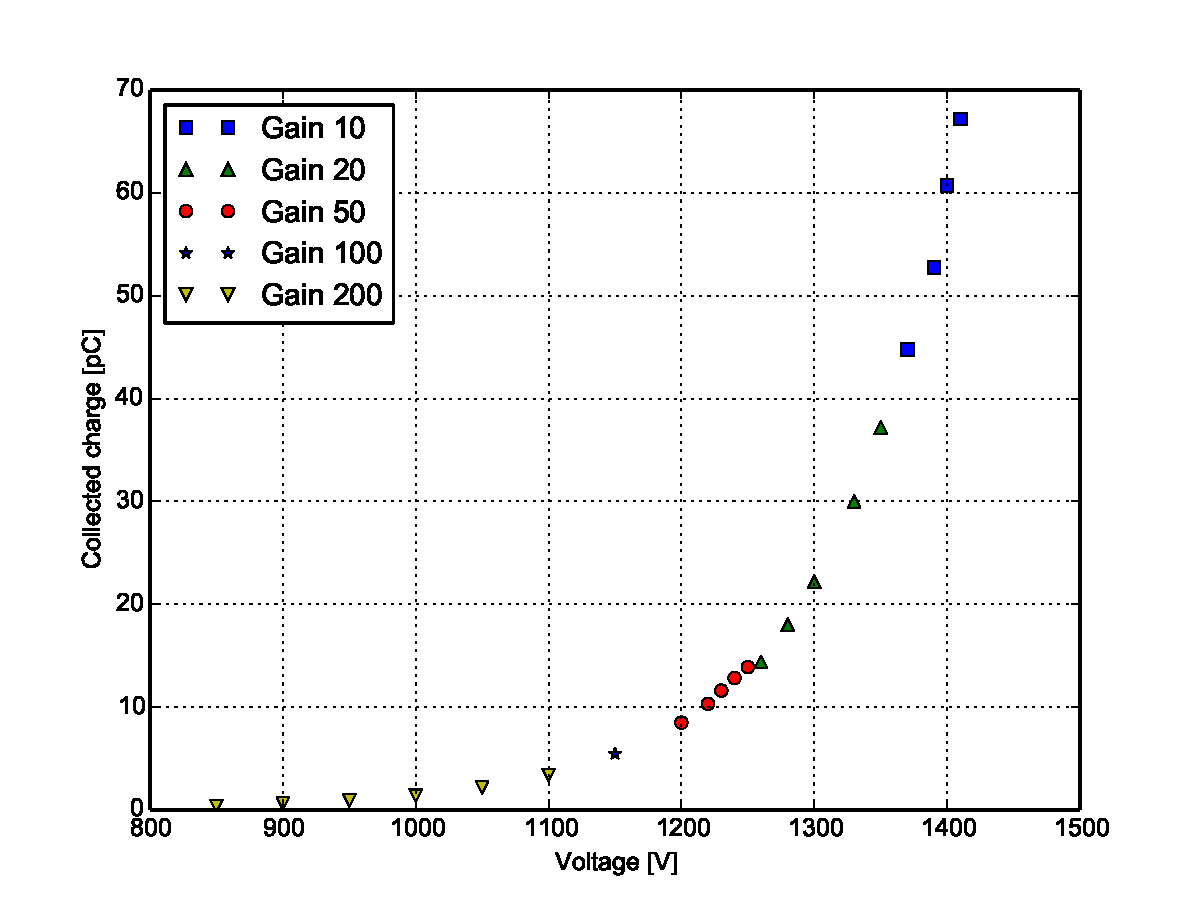
\includegraphics[width=\linewidth]{charge_vs_voltage}
    \caption{}
    \label{fig:charge_vs_voltage}
  \end{subfigure}
  \begin{subfigure}[t]{.48\linewidth}
    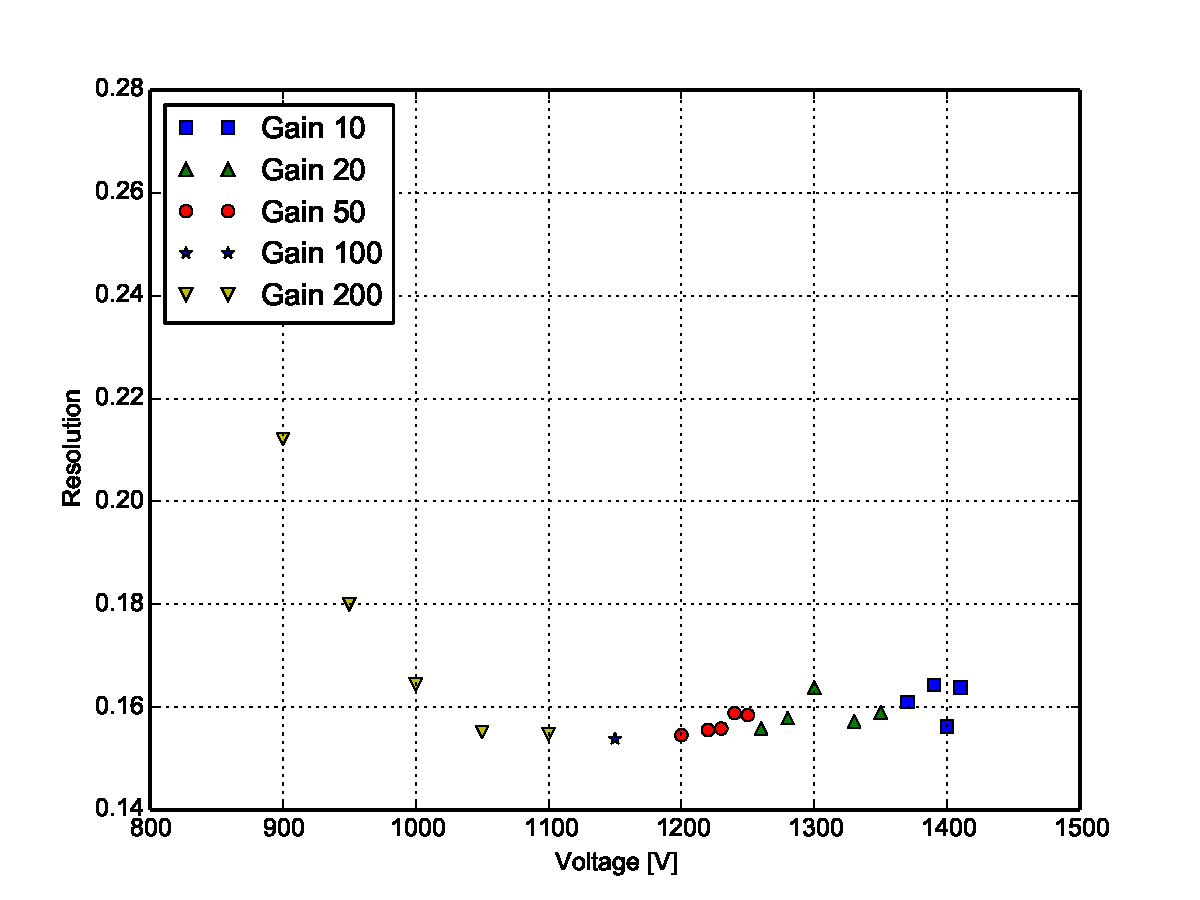
\includegraphics[width=\linewidth]{resolution_vs_voltage}
    \caption{}
    \label{fig:resolution_vs_voltage}
  \end{subfigure}
  \caption{}
  \label{fig:results}
\end{figure}
%%% Local Variables:
%%% mode: latex
%%% TeX-master: "prop_counter"
%%% End:
